
\chapter{Introduction}
\label{cha:introduction}

\texttt{PAFFS} stands for "Protective Aeronautics Flash FS" and aims to use a minimum RAM footprint with the ability to manage multiple flashes. Most of the design ideas are inspired by the file system \texttt{JFFS3} \referenceDocument{JFFS3}, which was later extended (\referenceDocument{JFFS3ex}) and discontinued as predecessor of \texttt{UBIFS}.\\
The main differences to usual disk file systems are \texttt{out-of-place-writing} and high deletion costs in terms of durability and speed. Keeping track of the files data chunks has to be different than just maintaining a big table on a disk, because the high frequented lookup table would be worn out earlier while other parts of flash will be nearly untouched. The standard approach of flash aware file systems (such as \texttt{YAFFS}) is to maintain a table-like structure in RAM and committing every chunk of new data to flash with an unique, increasing number, just like a list. This adds far more complexity to the file system as it has to scan the whole flash when mounting, but increases lifetime of the flash enormously. However, this RAM table grows linear with flash size, and thus does not scale for modern (> 2GB) flash chips. To solve this, the information has to be on flash. B+-Tree -> Section \ref{b+tree}.
Another big challenge is to reduce wear. Every change to data has to be written to another place and the old location has to be invalidated somehow. This is because the smallest unit of deletion is bigger (usually around 512 - 4086 times) than the smallest unit of a write operation. The common approach is to give every logical chunk an increasing version number. Because of the disadvantages pointed out earlier, this is not applicable to \texttt{PAFFS}. Areas and address mapping -> Section \ref{areas}

\section{Fundamental structures}
\label{sec:funst}

\subsection{Chained superblock}
\label{chainedSB}
\paragraph{Overview}
See \referenceDocument{JFFS3} chapter 4. Here will be a small overview.


\subsection{Areas}
\label{areas}
\paragraph{Overview}
\begin{itemize}
	\item To separate between different Types of Data
	\item \texttt{AreaType} can be one of Superblock, Index, Data, (Journaling)
	\item Address split in \texttt{logical area n°} and \texttt{page n°}, to give way for an easy garbage collector (see  fig. \ref{fig:area_address})
	\item \texttt{AreaMap} held in FLASH (but cached in RAM) translates between \texttt{logical area n°} and \texttt{physical area n°}
	\item \texttt{AreaMap} also keeps record of corresponding types and usage statistics for garbage collection
\end{itemize}

\paragraph{AreaTypes}
\begin{itemize}
	\item[Superblock] Superblock areas is automatically first\footnote{\texttt{\textbf{or first two, just to be sure?}}} area of flash. It contains the anchor area as well as jump pads and the superblock itself. See Chapter \ref{chainedSB}
	\item[Index] The index areas will contain only treenodes (including inodes). See Chapter \ref{b+tree}.
	\item[Data] Data areas contain data chunks of files, directories and softlinks referenced by the index.
	\item[Journal] The single Journal area (somewhen) will contain uncommited changes to the index.
\end{itemize}

\subsection{Tree Indexing}
\label{b+tree}
\paragraph{Overview}
B+Tree, minimum height. Is convenient when having to update whole path to root after a single node was changed. RAM Cache with parent pointers. Variable size, minimum Treeheight + 1\footnote{Check if true.}.

\section{Images}

\begin{figure}[ht]
  \centering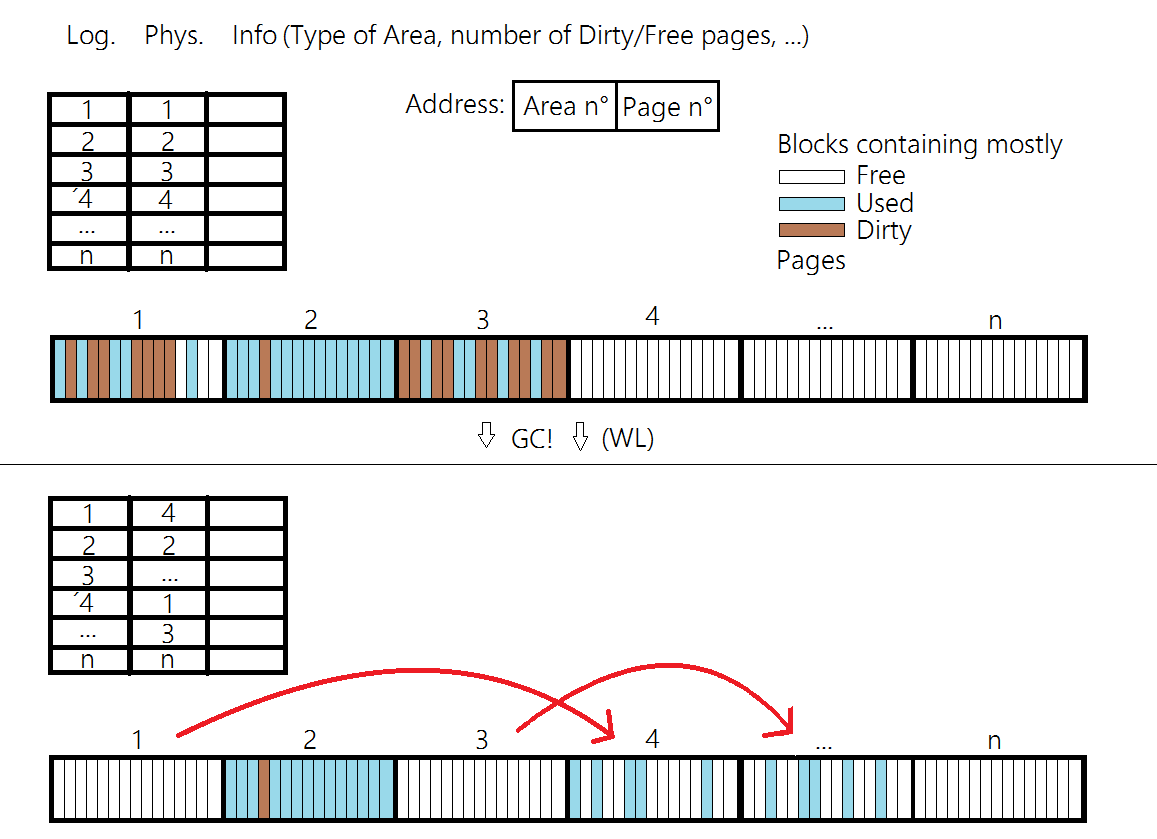
\includegraphics[width=\textwidth]{Areas_address.png}
  \caption{Basic process of garbage collection with areas}
  \label{fig:area_address}
\end{figure}
%
%\begin{figure}[htp]
%	\centering
%	\begin{subfigure}[t]{.49\textwidth}
%		\centering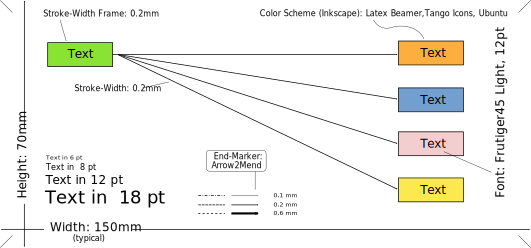
\includegraphics[width=7cm]{graphics_example}
%		\label{fig:graphics_example}
%		\subcaption{Example}
%	\end{subfigure}
%	\begin{subfigure}[t]{.49\textwidth}
%		\centering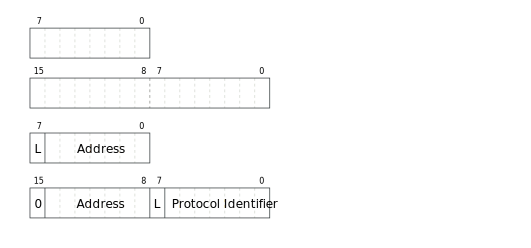
\includegraphics[width=7cm]{protocol_description_example}
%		\label{fig:protocol_example}
%		\subcaption{Protocol}
%	\end{subfigure}
%	\label{fig:images}
%	\caption{Two images side by side}
%\end{figure}


%\begin{lstlisting}[caption={Example C++ Code Listing},language=c++]
%enum TelemetryGeneration
%{
%    noTelemetry,
%    generateTelemetry
%};
%
%class Example
%{
%public:
%    Example(TelemetryGeneration telemetry,
%            uint8_t* buffer,
%            uint16_t length);
%    ...
%};
%
%Example object1(noTelemetry, 0, 0);
%
%uint8_t buffer[16];
%Example object1(generateTelemetry, buffer, size(buffer));
%\end{lstlisting}